%!TEX TS-program = pdflatex
%!TEX root = ../main.tex
%!TEX encoding = UTF-8 Unicode


\section[RESTfulDiner]{RESTfulDiner}

\subsection[System design]{System design}

\begin{frame}{Use Case Diagram}
	The first step of our development to identify the use cases of our system.
	We have identified four main use cases:

	\begin{figure}[h!]
		\centering
		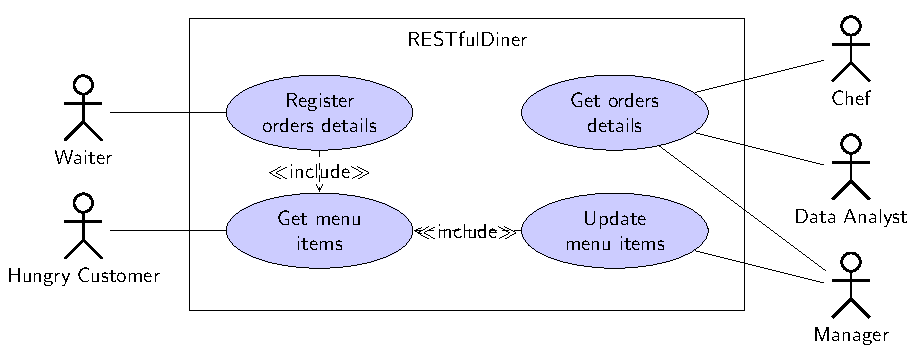
\includegraphics[width=0.9\textwidth,height=0.75\textheight,keepaspectratio]{images/usecases}
		\caption{Use cases diagram}
		\label{fig:usecases}
	\end{figure}

\end{frame}

\begin{frame}{E/R Diagram}
	\begin{figure}[h!]
		\centering
		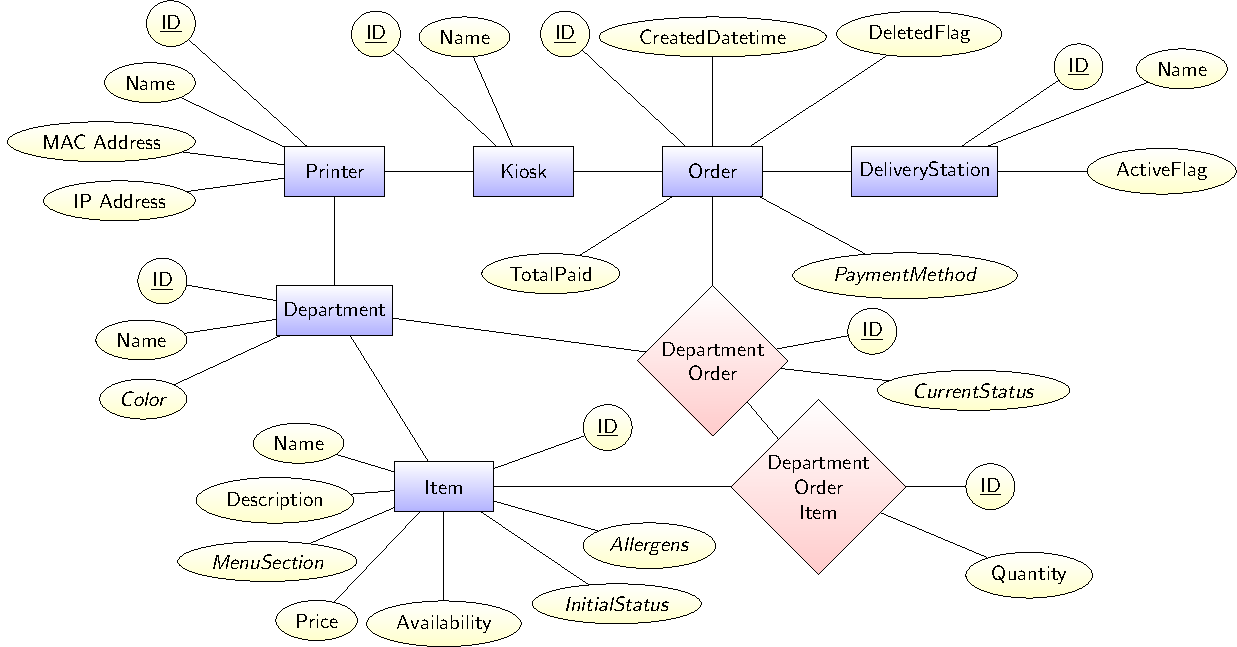
\includegraphics[width=\textwidth,height=0.75\textheight,keepaspectratio]{images/er}
		\caption{E/R diagram}
		\label{fig:er}
	\end{figure}

\end{frame}

\subsection[Open Data]{Open Data}

\begin{frame}[allowframebreaks]{Data model implementation}
	\lstinputlisting[style=PythonStyle,linerange={18-28}]{../app/models/_base.py}
	\lstinputlisting[style=PythonStyle,linerange={17-22,24-26,28-32,35-38}]{../app/models/department.py}
\end{frame}

\begin{frame}{API resources}
	\lstinputlisting[style=PythonStyle,linerange={12-12,16-33}]{../app/resources/department.py}
\end{frame}

\begin{frame}[fragile]
	\begin{lstlisting}[style=JSONStyle,caption={\texttt{GET /api/v1/departments} response}]
{
	"@context": {
		"schema": "https://schema.org/",
		"self": "@id",
		"type": "@type",
		"name": "schema:name",
		"printer": {
			"@id": "schema:isRelatedTo",
			"@type": "@id"
		},
		"license": {
			"@id": "schema:license",
			"@type": "@id"
		}
	},
	"license": "https://creativecommons.org/licenses/by/4.0/",
	"data": [
			{
			"self": "http://127.0.0.1/api/v1/departments/851c8de8-fb55-11ef-9aea-0242ac120003",
			"type": "schema:Organization",
			"name": "Kitchen",
			"printer": "http://127.0.0.1/api/v1/printers/67936882-fb55-11ef-b5b9-0242ac120003"
			},
		]
}\end{lstlisting}
\end{frame}

\begin{frame}[allowframebreaks]{Open Data principles}
	\begin{block}{\faStar\faStarO\faStarO\faStarO\faStarO}
		Make your stuff available on the Web (whatever format) under an open
		license.
	\end{block}
	\begin{block}{\faStar\faStar\faStarO\faStarO\faStarO}
		Make it available as structured data (e.g., Excel instead of image scan
		of a table).
	\end{block}
	\begin{block}{\faStar\faStar\faStar\faStarO\faStarO}
		Make it available in a non-proprietary open format (e.g., CSV instead of
		Excel).
	\end{block}
	These requirements are satisfied by our RESTful API that allows
	publicly access to data in JSON format and provide them under Creative
	Commons license.

	\begin{block}{\faStar\faStar\faStar\faStar\faStarO}
		Use URIs to denote things, so that people can point at your stuff.
	\end{block}
	\begin{block}{\faStar\faStar\faStar\faStar\faStar}
		Link your data to other data to provide context.
	\end{block}
	Every resource in the system is identified by a URI, and can be accessed
	by a simple HTTP GET request to that URI. A relation between resources
	is established by linking them in the JSON response.
\end{frame}
